%% The following is a directive for TeXShop to indicate the main file
%%!TEX root = diss.tex

\chapter{Results}
\label{ch:Results}
\section{Particle Identification}
\label{sec:particleIdentification}
In order to identify particles using the \ac{ARICH} detector, a particle likelihood method is used \cite{richImpact, belleArich}.
For this method, we take the measured momentum of the particle, and use Equation \TODO{Include relativistic equation for mass / momentum / velocity here } to determine the expected velocity for different candidate particles masses.
The candidate particles of interest for this study are protons, pions, and kaons.
For each velocity hypothesis, we run 10,000 simulations of particles moving at that velocity, with the same measured initial trajectory as input, and get the distribution of the resulting photons.
For each pixel of the detector, this procedure will give a value $\lambda_i(\beta)$, equal to the expected number of photons striking pixel $i$ in the detector due to a particle of velocity $\beta$. 

For a given experimental event, we will detect $N_i$ photons in each pixel $i$.
In reality, the PMTs are only capable of registering whether or not a photon has been detected - if multiple photons strike a single pixel in a very short amount of time, it will not be able to distinguish the number detected, so we just know if $N_i = 0$ or $N_i > 0$.

If we assume that the number of photons striking detectable by a PMT pixel is given by a Poisson distribution, then the probability that zero photons strike pixel $i$ is given by:
$$ P_i(N_i=0; \beta) = e^{-\lambda_i(\beta)} $$
 The probability that one or more photons strike pixel $i$ must then be:
$$ P_i(N_i>1; \beta) = 1 - e^{-\lambda_i(\beta)} $$

By multiplying the probabilities of getting the observed result in each pixel $i$ of the detector, we calculate the likelihood for that value of $\beta$:

$$L_\beta = \prod_{i}P_i(N_i; \beta)$$

Because the log function is montonic, instead of maximizing the likelihood function, we can instead minimize the negative log-likelihood, which is easier to compute:
\begin{equation}
    \label{eq:loglikelihood}
    -2\ln(L_\beta) = -2\sum_i \ln(P_i(N_i; \beta))
\end{equation}

\TODO{Due to the relatively high error associated with the measurement of the particle momenta, if I find that this method is not entirely sufficient at identifying particles then I will enhance the technique by scanning over different momentum hypotheses. This has not yet been implemented}

\section{Multi-particle events}
\TODO{In this section, I will  talk about multi-particle events. It is often the case that the photons from several different particles will be detected at the same time. The resulting photon distributions cannot necessarily be disentangled, so I will have to look at how to fit both particles at once. This has not yet been implemented.}


\section{Particle Separation}
In this section, I will talk about how well the likelihood approach using my simulation differentiates between different particles. 
Charged pions have a mass of  0.140 GeV, charged kaons have a mass of 0.494 GeV, and protons have a mass of 0.938 GeV.
Because of this, it is particularly hard to distinguish between pions and kaons, but easier to distinguish protons from kaons, and easier still to distinguish protons from pions.

Let's suppose we want to see how well this likelihood approach works on a particle that is 7 GeV and measured to be at the origin and travelling directly in the z-direction.
To check the certainty with which we can determine whether this is a pion or kaon, we would follow this approach:

\begin{enumerate}
\item Generate 10,000 pions with these values in Geant4, project the generated photons onto a detector, apply efficiency corrections, and store the resulting histogram of detected photon hits for each pion. 
\item Do the same, but with kaons instead of pions
\item Given the particle initial position, initial direction, and momentum, we use my simulation to generate two photon probability distribution histograms, corresponding to pions or kaons
\item For each event simulated in Geant4, we compute the log likelihood of the histogram with respect to each of the 3 photon probability distribution functions.
\item For each true particle type, we plot a histogram of the log of the ratio of likelihoods between the two hypotheses.
This is just the differences between the log-likelihoods of the two hypotheses.
\item We look at the separation between the distributions: this is equal to the difference in means between the distributions, divided by the RMS of each distribution added in quadrature
\end{enumerate}

The result of this procedure is shown in Figure \ref{fig:kaonpionsep}. The two distributions are separated by a distance of $2.4 \sigma$ - the significant overlap between the two distribution indicates that there is a relatively high chance of misidentification. Applying the same procedure to verify our separation between kaons and protons gives the results shown in Figure \ref{fig:kaonprotonsep}. Here we see that the two distributions do not significantly overlap and have a separation of $4.7 \sigma$, meaning that at this momentum and angle, protons are very unlikely to be misidentified as kaons, and vice versa.
\begin{figure}[]
\centering
\resizebox{0.9\textwidth}{!}{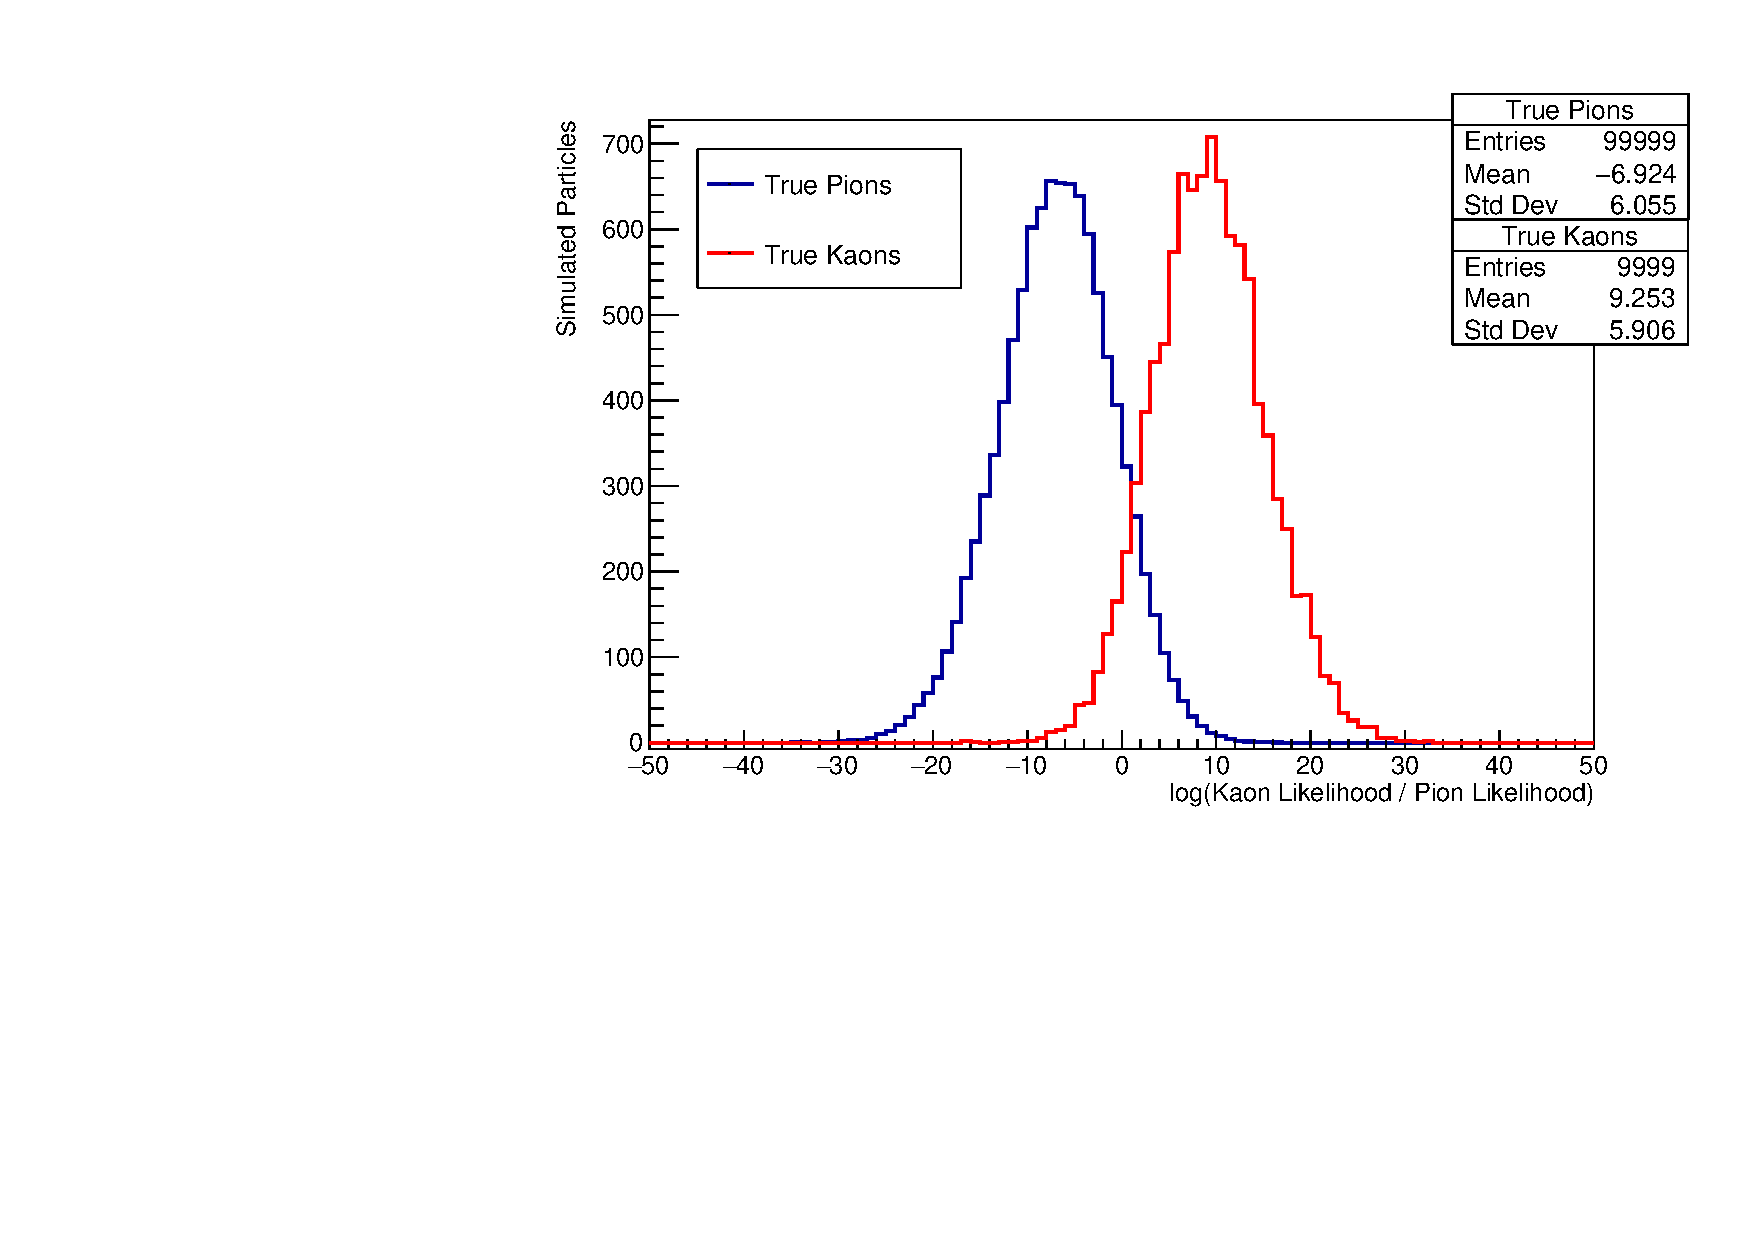
\includegraphics{./figs/kaonPionSep.pdf}}
\caption[Particle identification separation for 7 GeV pions and kaons]{Histogram showing the logarithm of the ratios of likelihoods between kaons and pions for both ``true" kaons and ``true" pions. The two distributions have a separation of 2.4 $\sigma$.}
\label{fig:kaonpionsep} 
\end{figure}

\begin{figure}[]
\centering
\resizebox{0.9\textwidth}{!}{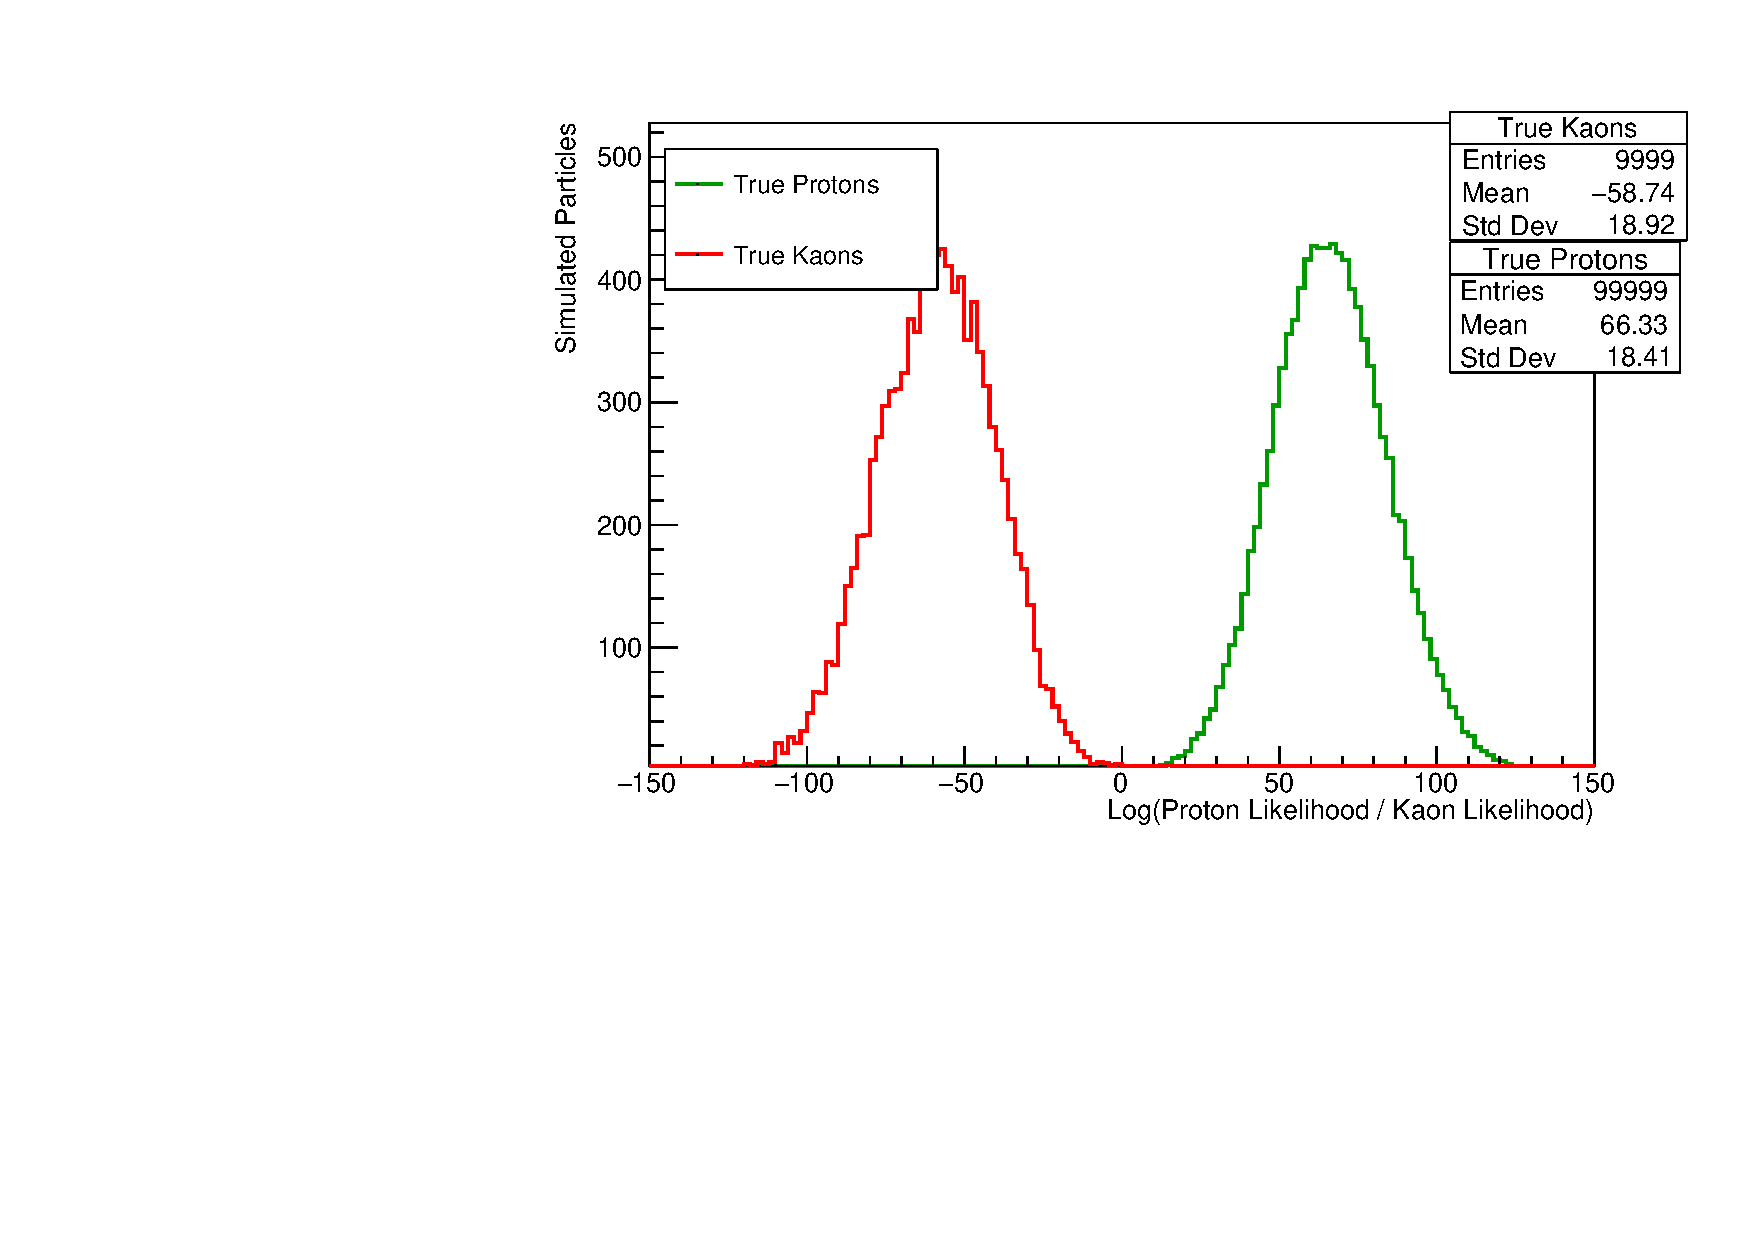
\includegraphics{./figs/kaonProtonSep.pdf}}
\caption[Particle identification separation for 7 GeV kaons and protons]{Histogram showing the logarithm of the ratios of likelihoods between protons and kaons for both ``true" protons and ``true" kaons. The two distributions have a separation of  4.7 $\sigma$.}
\label{fig:kaonprotonsep} 
\end{figure}

\TODO{While I have examined these results for 7 GeV pions, kaons, and protons, I still must check the separation for: \\
- Different initial particle directions and positions \\
- Different momenta \\
- Multi-particle events
}

\endinput

Any text after an \endinput is ignored.
You could put scraps here or things in progress.
